\taskpic{Длинная тяжелая и гибкая веревка с массой $\rho$ на единицу
  длины натянута с постоянной силой $F$. Внезапное движение формирует
  круглую петлю на одном конце веревки, и петля бежит по веревке с
  некоторой скоростью $c$, как показано на рисунке. Вычислите
  $c$.}{
  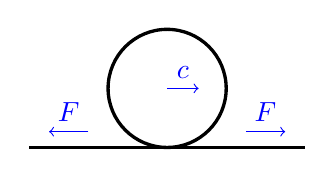
\begin{tikzpicture}
    \draw[very thick] (0.25,0) -- (3.75,0);
    \draw[very thick] (2,0.75) circle (0.75cm);
    \draw[blue,->] (1,0.2) -- ++(-0.5,0) node[midway,above] {$F$};
    \draw[blue,->] (3,0.2) -- ++(+0.5,0) node[midway,above] {$F$};
    \draw[blue,->] (2,0.75) -- ++(0.4cm,0) node[midway,above] {$c$};
  \end{tikzpicture}
}
